% Täällä kerrotaan aikaisemmista, vastaavista projekteista

\section{Aikaisempia opetuskäyttöön suunnattuja järjestelmiä}

\fxnote{
Basic 1964\\
Logo 1967\\
Pascal 1960-1970\\
C 1972, kulta-aika 1990-luvulla\\
Java 1995\\
Scratch 2006
}

Kautta tietojenkäsittelytieteen
opettamisen historian ohjelmoinnin
opettamiseen on kehitelty
monia erilaisia ohjelmointikieliä.
Tässä luvussa esittelen muutamia
historiallisesti merkittäviä
ohjelmointikieliä, joita
on käytetty ohjelmoinnin opettamiseen.
Lähes kaikki ensimmäisistä
ohjelmointikielistä olivat
tekstipohjaisia, eli
niitä ei ollut suunniteltu
graafisten ohjelmien,
kuten pelien, tekmiseen.
Lisäksi esittelen myös muutamia uusia
ohjelmointikieliä, jotkai toimivat
EppaBasicin tavoin selainympäristössä.

Eräs ensimmäisistä ohjelmoinnin
opettamiseen kehitetyistä
ohjelmointikielistä oli
Dartmouth Collegessa vuonna 1964
kehitetty BASIC.
BASIC kehitettiin erityisesti
opiskelijoille, joilla ei ollut
matemaattisluonnontieteellistä
taustaa.
Alkuperäinen BASIC oli hyvin
rajoittunut, mutta myöhemmät
murteet ovat tuoneet mukanaan
kieleen uusia ominaisuuksia.
Myös EppaBasic on
tällainen murre.
Muita merkittäviä BASIC-murteita
ovat esimerkiksi
Microsoftin kehittämä
Visual Basic ja
Jukka Lavosen kehittämä
CoolBasic, joka on inspiroinut
myös EppaBasicin kehitystyötä.

Ohjelmointikielet, jotka ovat
toistensa murteita,
muistuttavat rakenteeltaan
toisiaan.
Murteet eivät välttämättä
ole yhteensopivia keskenään,
joten niitä voidaan kutsua
myös omiksi kielikseen.
Tästä syystä murteilla
usein onkin omat nimensä.

Eräs ensimmäisistä ohjelmointikielistä,
jolla pystyi tekemään grafiikka,
oli vuonna 1967 kehitetty Logo.
Se muistetaan erityisesti
"kilpikonna-grafiikastaan",
jossa ohjelmakomennoilla
siirretään kilpikonnaa,
joka piirtää kulkiessaan
näytölle viivan.
Logo pohjautuu vuonna 1958
julkaistuun Lisp-ohjelmointikieleen.

Vuonna 1970 Niklaus Wirth
julkaisi Pascal-ohjelmointikielen.
Kieli suunniteltiin erityisesti
opetuskäyttöön, ja se yhdisti
aikansa yleisimpien ohjelmointikielten
parhaat ominaisuudet samalla
karsien epäsäännönmukaisuuksia
\cite{language_history}.
Pascal oli yritysten käytössä aina
1990-luvulle asti, kunnes C
syrjäytti sen.

2000-luvulle tultaessa alkoi
verkkoselainten kehittyessä
ilmestyä ohjelmointikieliä
myös selainympäristöön.
Tällaisille kielille on tyypillistä,
että niillä voi helposti luoda
ainakin yksinkertaista grafiikkaa.

Eräs selainympäristössä toimiva
ohjelmointikieli on Massachusetts
Institute of Technologyn kehittämä
Scratch-ohjelmointikieli
(ks. Kuva \ref{img:scratch}).
Scratch on graafinen ohjelmointikieli,
mikä tarkoittaa sitä, että
kieltä ohjelmoidaan raahaamalla
hiirellä komentopalikoita
ohjelmointialueelle.

OPS 2016 -dokumentissa mainitaan,
että perukoulun ensimmäisillä
luokilla on tarkoitus käyttää
muun muassa graafisia ohjelmointikieliä.
Myöhemmillä luokilla on tarkoitus
harjoitella hyviä ohjelmointikäytöntöjä,
mikä käytännössä tarkoittaa siirtymistä
tekstuaalisiin ohjelmointikieliin
eli ohjelmoitikieliin, joita ohjelmoidaan
kirjoittamalla koodia.
EppaBasic on yksi mahdollisuus
yläluokilla käytettäväksi ohjelmointikieleksi,
mutta käyttö alaluokilla on myös mahdollista.
\fxnote{Tarkista OPS 2016 ja lisää viite}

\begin{figure}[h]
    \centering
    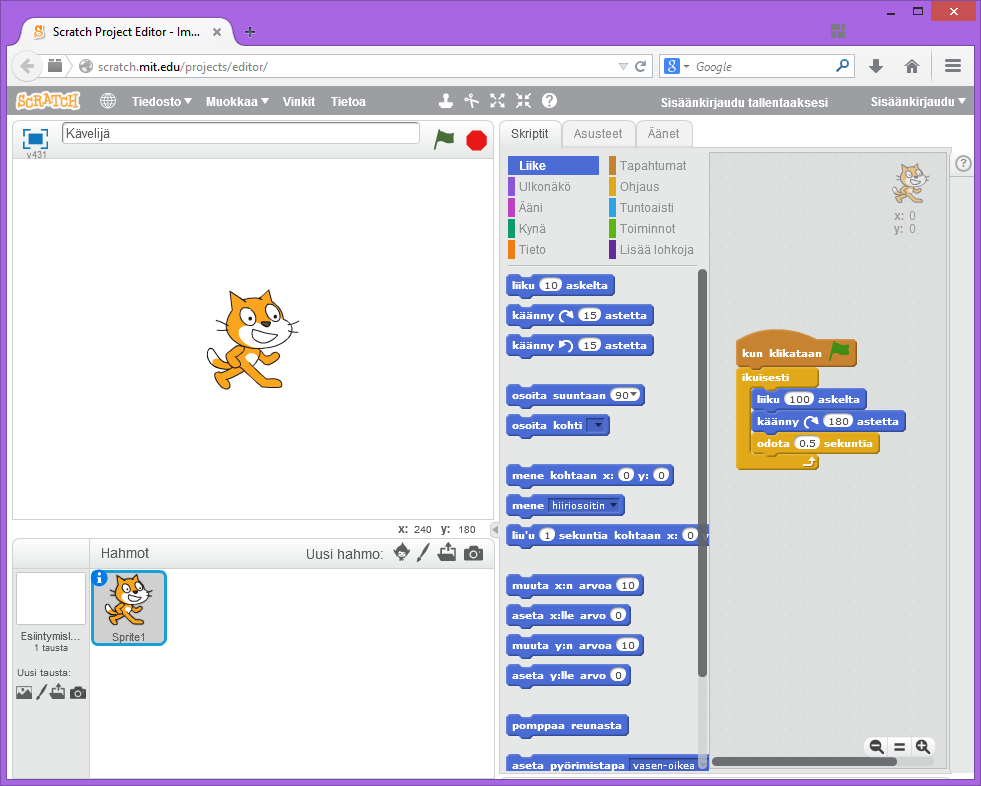
\includegraphics[width=1\textwidth]{scratch}
    \caption{Scratch-ohjelmointiympäristö, jossa vasemmassa yläkulmassa suoritusalue ja oikealla ohjelmointialue, jossa lyhyt ohjelmakoodi.}
    \label{img:scratch}
\end{figure}


\begin{comment}
Monia kieliä on käännetty selainympäristöön
(esim. \eng{Python}, \eng{Lua}) \cite{repl.it}
Näillä kielillä grafiikan luominen on kuitenkin usein hankalaa.
Lisäksi useissa toteutuksissa ohjelmien on oltava lyhyitä,
sillä ohjelman suorittaminen jäädyttää selaimen,
kunnes ohjelma on suoritettu kokonaisuudessaan.
\fxnote{Esimerkkejä}

On myös kehitetty erilaisia ohjelmoinnin aloittelijoille suunnattuja,
selainympäristössä toimivia ohjelmointikieliä,
kuten esimerkiksi Massachusetts Institute of Technologyn
kehittämä Scratch-ohjelmointikieli.
\fxnote{Tarkista MIT ja Scratch}
Scratch on graafinen ohjelmointikieli,
mikä tarkoittaa,
että sen ohjelmoiminen tapahtuu raahamalla erilaisia komentopalikoita
peräkkäin ja sisäkkäin.
Vaikka tämä onkin nopeasti omaksuttava tapa tehdä omia ohjelmia,
suurien ohjelmien tekeminen on hankalaa,
samoin kuin siirtyminen myöhemmin muihiin kieliin.
Scratch on mielestämme liian rajoittunut kieli
yli kymmenvuotiaille nuorille.

\fxnote{Varmista sivu ja lisää linkki}
Codeacademy on tarjoaa omaa selaimessa toimivaa ohjelmointiympäristöään.
Kyseisessä ympäristössä ohjelmoidaan \eng{JavaScript}-kielellä,
joka muistuttaa läheisesti muita yleisesti käytettyjä kieliä,
kuten Java ja C++.
Ympäristössä syötteiden lukeminen ja piirtäminen
tapahtuu tapahtumien (eng. \eng{Events}) perusteella.
Mielestämme tapahtumien käyttäminen luo kuitenkin ohjelmakoodiin
aloittelijoille hankalasti ymmärrettävän suoritusjärjestyksen,
sillä koodin suoritus hyppii tapahtumien ohjelmarunkojen välillä.
\fxnote{Parempi sana}
Tämän takia oma ohjelmointikielemme rakenne ei pohjaudu eventteihin
vaan ohjelmakoodi suoritetaan aina ohjelmoijan kannalta loogisessa,
deterministisessä järjestyksessä.
\end{comment}

\fxnote{Älä hauku! Basiceista, Pascalista, Logosta... muista aloituskielistä}
